\documentclass{article}
\usepackage{graphicx}
\usepackage{ulem}
\usepackage{fullpage}
\usepackage{tocloft}
\usepackage{graphicx}
\usepackage{hyperref}
\usepackage{amsmath}
\usepackage{tcolorbox}
\usepackage{xcolor}
\usepackage{subcaption}
\usepackage{animate}
\usepackage{url}
\usepackage{natbib}

\setcounter{tocdepth}{2}
\begin{document}

\begin{titlepage}
	\centering
	{\scshape\Large \uline{\hspace{12cm}}\par}
	{\scshape\Large \uline{GoDaddy - Microbusiness Density Forecasting}\par}
	\vspace{1cm}
	
\includegraphics[width=0.35\textwidth]{images/iitgoa-logo.png}\par\vspace{1cm}
	\vspace{1cm}
	{\Large\itshape Submitted by\par}
	\vspace{0.5cm}
	{\Large Mahendra Kumar\par}
	\vspace{1cm}
	{\Large\itshape Under the guidance of \par}
	\vspace{0.5cm}
	{\Large Dr. Saurabh Trivedi\par}
	\vspace{2cm}
	{\Large School of Mathematics and Computer Science\par}
	\vspace{0.5cm}
	{\Large Indian Institute of Technology, Goa\par}
	\vfill
	{\large \today\par}
\end{titlepage}
\renewcommand\contentsname{Table of Contents\vspace{1cm}}
\begin{center}
	\tableofcontents
\end{center}
\cftsetpnumwidth{2em}
\newpage

\section{\centering Introduction}
\vspace{1em}
The project aims to investigate the effectiveness of time series forecasting techniques on real-world dataset provided by a kaggle competition, \textit{GoDaddy - Microbusiness Density Forecasting} \cite{kaggle_competition} . The micro-business density of an area is defined as number of active micro-businesses ( businesses with less than 10 employees) per 100 people over the age of 18 in given county. This Kaggle competition is conducted by GoDaddy, a company that provides small businesses domain registration, web hosting, and other online services. The competition aims to develop machine learning models that can accurately forecast the micro-business density in different areas/counties of the United States. 

\paragraph{Motivation} Microbusiness density data can be a powerful tool for policymakers to support small businesses and promote economic growth and development in their communities. By leveraging this data, policymakers can make more informed decisions about how to allocate resources and develop policies that meet the needs of their constituents.

\paragraph{} Microbusinesses, due to their small size and relative newness, often do not appear in traditional economic data sources. However, their activity may exhibit correlation with other economic indicators that are of general interest.For the competition, GoDaddy provided two types of data for each county in the US, which are micro-business density data and census data. 

\vspace{2em}
\section{\centering Data Overview}
\vspace{1em}
GoDaddy has provided the microbusiness density data from August 2019 to December 2023 for analysis. The microbusiness density of each county is updated monthly at the start of every month. The data contains the microbusiness density of 3135 counties in the US. Also, for each county, yearly census data is given, which includes five economic indicators: 

\begin{itemize}
\item \textit{pct\_bb} -  percentage of broadband connections
\item \textit{pct\_college} - percentage of individuals with a 4-year college degree 
\item \textit{pct\_foreign\_born} - percentage of foreign-born individuals in the population
\item \textit{pct\_it\_workers} - percentage of the workforce in the county employed in information related industries
\item \textit{median\_hh\_inc} - median household income
\end{itemize}

\begin{figure}[ht]
	\centering
	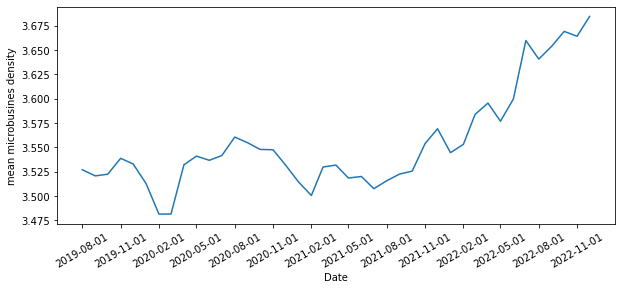
\includegraphics[width=0.5\textwidth]{images/mbd_gif/time_variation}
	\caption{Mean microbusiness density variation in US}
	\label{fig:fig1}
\end{figure}

\vspace{1em}
\paragraph{Observation}  Figure \ref{fig:fig1}  indicates over the last three years mean microbusiness density of the whole US has increased, denoting an increase in online stores in the US.

\vspace{2em}
\section{\centering Data Analysis}

Data analysis is the process of systematically examining and interpreting data to extract useful insights, identify patterns and trends, and draw conclusions from it. Clustering is one such technique. 

\subsection{Clustering}

\paragraph{Definition} Clustering is the process of grouping similar objects or data points together based on their characteristics or attributes. It is a unsupervised learning technique that involves identifying patterns and structures in data without a priori knowledge of the groups or categories.

\begin{figure}[h]
	\centering
	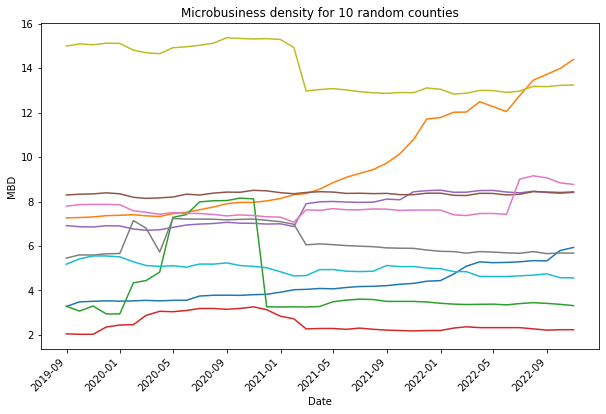
\includegraphics[width=0.4\textwidth]{images/random10}
	\caption{Microbusiness density of some counties}
	\label{fig:fig2}
\end{figure}

\paragraph{Observation} In Figure \ref{fig:fig2}, We see the microbusiness-density plot is not smooth and this may interfere with the clustering algorithm described in the next section. To avoid that, we use a technique, \textit{savitzky-golay filtering} algorithm.

\subsubsection{Savitzky-Golay Filtering}
Savitzky-Golay Filtering is a smoothing technique used for time series data. It works by fitting a polynomial of a certain degree to the window of consecutive data points and then using this polynomial to estimate the smoothed values at the center point of the window. The polynomial coefficients are chosen to minimize the squared error between the polynomial and data points within the window. The filter is also helpful in preserving essential features of the data, such as peaks and valleys, while still smoothing out the noise. 

\subsubsection{DBSCAN Algorithm}
DBSCAN is an acronym for \textbf{density-based spatial clustering of application with noise} is an algorithm for clustering. This clustering algorithm groups similar points in a dataset based on their density.  
The algorithm defines a neighborhood around each point in the dataset and then identifies clusters as areas of high density. The neighborhood is defined by two parameters \textbf{\textit{eps}}, which specifies the maximum distance between two points to be considered neighbors, and \textbf{\textit{min\_samples}}, which specifies the minimum number of points required to form a dense region. 

\vspace{1em}
The algorithm starts by selecting an arbitrary point and identifying all its neighbors within a distance of eps. If the point has at least min\_samples neighbors, it is considered a core point, and a new cluster is formed around it. The algorithm then expands the cluster by iteratively adding all neighboring points, as long as they have at least min\_samples neighbors. Once there are no more points to add, the algorithm selects a new unvisited point and repeats the process until all points have been visited.

\vspace{1em} 
Points that are not part of any cluster are considered \textbf{\textit{noise\_points}}. These points are either too far away from any cluster to be included or have fewer than min\_samples neighbors.

\vspace{1em}
DBSCAN has some advantages over other clustering algorithms such as K-means. It can handle non-linearly seperable data and does not require the user to specify the number of clusters beforehand. However it can be sensitive to choice of parameters eps and min\_samples, and clustering results may vary depending on dataset and the parameter values chosen.

\subsubsection{Results and Observations}

\begin{figure}[h]
	\centering
	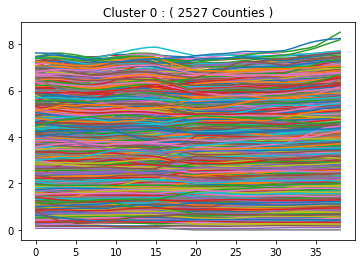
\includegraphics[width=0.3\textwidth]{images/cluster0}
	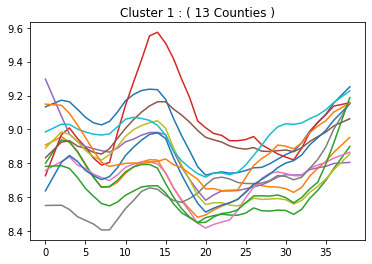
\includegraphics[width=0.3\textwidth]{images/cluster1}
	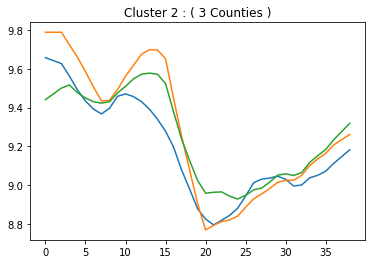
\includegraphics[width=0.3\textwidth]{images/cluster2}
	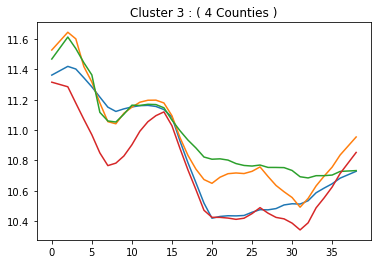
\includegraphics[width=0.3\textwidth]{images/cluster3}
	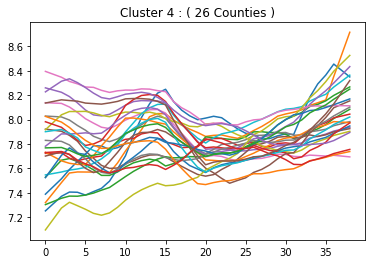
\includegraphics[width=0.3\textwidth]{images/cluster4}
	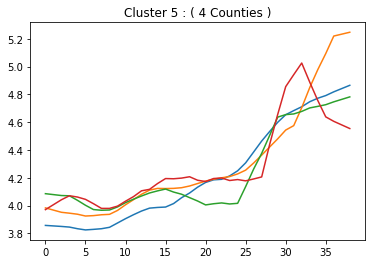
\includegraphics[width=0.3\textwidth]{images/cluster5}
	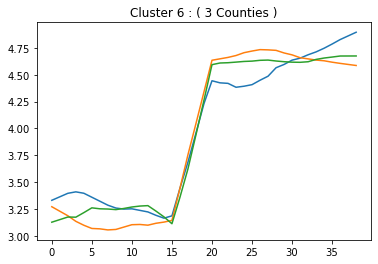
\includegraphics[width=0.3\textwidth]{images/cluster6}
	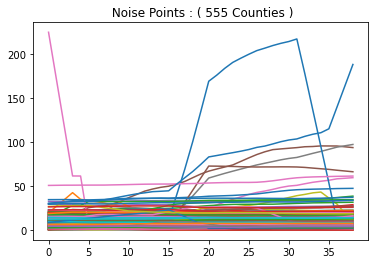
\includegraphics[width=0.3\textwidth]{images/noise}
	\caption{Clusters generated by DBSCAN Algorithm with \textbf{eps} = 1 and \textbf{min\_samples} = 3}. X-axis shows the time and Y-axis shows the microbusiness density. different colors indicate different counties. 
\end{figure}

\textbf{Note: }Parameters for the savitzky-golay filtering and the dbscan algorithm are chosen after manually finding clusters for various parameter values and visually inspecting results. 

\vspace{1em}
Before clustering, we applied savitzky-golay filtering with \textbf{window\_size 3} and\textbf{ polynomial\_order 1}, which is simply moving average smoothing. As we can see, nearly 80\% counties fall into Cluster 0. It is happening because, for these counties, micro-business density is mostly the same, and so they form a cluster. Also, nearly 500 counties are noise points, i.e., they do not fall into any cluster. 

\subsection{Time Series Splitting}

\vspace{1em}
Irrespective of type of model being used, we will use 90\% data for training and 10\% data for validation. Also we will retrain model on whole data before making prediction on test data ( i.e. making predictions of microbusiness density for upcoming months ) which is hidden. The reason for this is that when we split data into train and validation sets, we are reserving a portion of data for evaluating the performance of model. This means that your model has not seen this data during training, and therefore, it may not be optimized to make predictions on this new unseen data.

\vspace{1em}
By retraining the model on the entire training dataset, we are incorporating the information from both the original training data and the validation data into the model. This can help to improve the generalization performance of the model, as it has seen more data during
training.

\vspace{1em}
In traditional machine learning, we can split data randomly into training, validation, and test sets, but for time series, data must be split \textit{chronologically}, i.e., in order of time. It is because time series data has a temporal component meaning past observations influence future ones. Therefore, evaluating the model’s performance on data it has not seen before is essential. 

\vspace{1em}
Machine learning algorithms like linear regression, random forest, and xgboost, expect the input to be one-dimensional so we can directly feed microbusiness density data into the model and make predictions. However, in most deep learning algorithms that use convolutional neural networks (CNN) or recurrent neural networks (RNN), we must convert data into a 2-dimensional array with input-output pairs. To convert a time series into a 2-D array, we can use the \textbf{\textit{time series split}} methodology explained below.

\vspace{1em}
\begin{figure}[h]
	\centering
	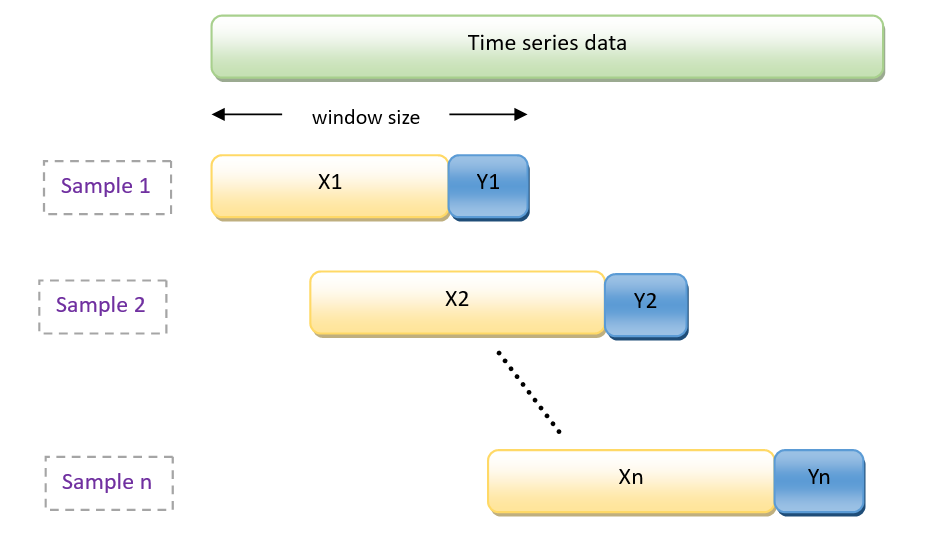
\includegraphics[scale=0.6]{images/timeseriessplit}
	\caption{Time Series Split}
\end{figure}

For each county in US, first we transform one-dimensional (1-D) microbusiness data into two-dimensional (2-D) data using a window of length window size and sliding it over 1-D data. In each window, we take last value as output and remaining elements as input.

\vspace{2em}
\section{\centering Evaluation Criterion}
\vspace{1em}
In this competition, submissions are evaluated on \textit{SMAPE} between forecasts and actual values. 

\subsection{SMAPE}
SMAPE is an acronym for \textbf{symmetric mean absolute percentage error} is an evaluation metric used in forecasting to measure the accuracy of the predicted values compared to the actual values. It is defined as:

\vspace{1em}
\begin{equation*}
	\text{SMAPE} = \frac{1}{n} \sum_{t=1}^n \frac{|F_t - A_t|}{(|F_t| + |A_t|)/2},
\end{equation*}

\vspace{1em}
where $F_t$ is the forecasted value for time period t, $A_t$ is the actual value for time period t, and n is the number of time periods being evaluated. 

\begin{figure}[h]
	\centering
	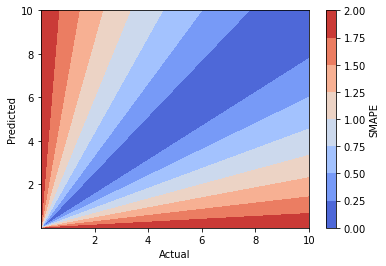
\includegraphics[scale=0.5]{images/smape_contour}
	\caption{Contour plot of SMAPE values}
\end{figure}

\vspace{1em}
The SMAPE formula computes the percentage difference between the actual and forecasted values, and then takes the average of these differences, giving equal weight to each time period. The SMAPE value ranges between 0 and 2 , where a value of 0 indicates a perfect forecast and a value of 2 indicates a forecast that is completely wrong.

\vspace{2em}
\textit{Now we see performance of various time series forecasting techniques on given dataset}

\section{\centering Baseline Model - Linear regression}

\vspace{1em}
\textbf{Linear regression} is a statistical method used to analyze the relationship between a dependent variable  (also called the response variable)  and one or more independent variables (also called the predictor or explanatory variables). Intuitively, linear regression tries to find a line that best represents the relationship between the independent and dependent variables. In this competition, we have used following linear equation: 

\vspace{1em}
\begin{center}
\begin{tcolorbox}[colframe=orange,boxsep=5pt,boxrule=1pt,colback=white, width=0.7\linewidth]
$
Y_t = \beta_0  + \beta_1 * x_{1,t} + \beta_2 *  x_{2,t}  + \beta_3 * x_{3,t} +  \beta_4 * x_{4,t} + \beta_5 * x_{5,t} + \varepsilon_t 
$
\end{tcolorbox}
\end{center}

\vspace{1em}
\begin{itemize}
	\item $Y_t$ is the observed value of the microbusiness-density at \textit{time\_step} t
	\item $\varepsilon_t$ is error term at \textit{time\_step} t
	\item $x_{1,t}, \ldots , x_{5,t}$ denotes \textit{pct\_bb}, \textit{median\_hh\_inc}, \textit{pct\_college}, \textit{pct\_foreign\_born} and  \textit{pct\_it\_workers} respectively at \textit{time\_step} t
\end{itemize}
\vspace{1em}

\subsection{Objective}

The error or residual term, $\varepsilon_t$ represents the difference between the actual response variable value and the predicted value from the linear regression model. By minimizing the sum of the squared errors or residuals (SSE), linear regression seeks to reduce the variance of the errors or residuals and thereby explain as much of the variation in the response variable as possible using the predictor variable(s) in the model.

$$
	SSE = \frac{\sum_{t=0}^{n} \varepsilon_t^2}{n}
$$

To find the values of $\beta_0 \ldots \beta_5$, linear regression uses the ordinary least square method, which takes the partial derivative of SSE w.r.t. each coefficient. Thus we get k (here k=6) equations and k unknowns. This system of equations can be solved to get a closed-form solution given by 

$$
\hat{\beta} = [ \beta_0 \ldots \beta_5 ] = (X^TX)^{-1}X^TY
$$

 
Where 

\vspace{1em}

\begin{center}
	\begin{minipage}{0.45\linewidth}
		\[
		X = \begin{pmatrix}
			x_{1,1} & \cdots & x_{5,1} \\
			\vdots  & \ddots & \vdots \\
			x_{1,n} & \cdots & x_{5,n} \\
		\end{pmatrix}
		\]
	\end{minipage}
	\begin{minipage}{0.45\linewidth}
		\[
		Y = \begin{pmatrix}
			Y_1 \\
			\vdots \\
			Y_n \\
		\end{pmatrix}
		\]
	\end{minipage}
\end{center}

\vspace{1em}
\subsection{Results and Observations}

\vspace{1em}
\begin{figure}[h]
	\centering
	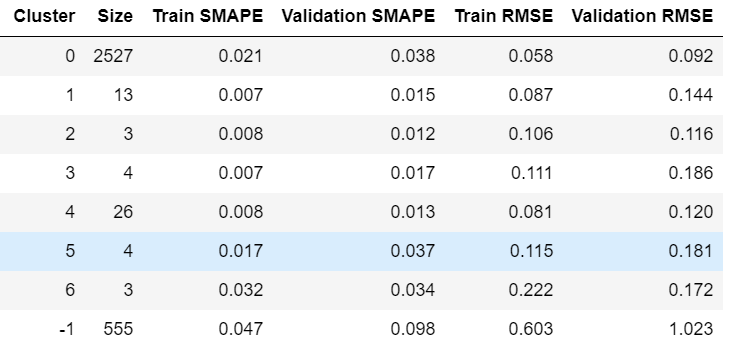
\includegraphics[width=0.8\linewidth]{images/lr_results}
	\caption{LR model performance on each cluster}
\end{figure}

\textbf{Note}: \textit{Throughtout my analysis I have used 2\% smape error as threshold for permissible error} 

After analyzing the Linear regression results, we saw that \textbf{930 counties} have validation smape error of less than 2\%. But when we made just one modification, training linear model on the last year's data after covid, i.e., 2022, we see the number of counties with validation smape error less than 2\% jumps to \textbf{2238 counties}. It happened because, due to covid, many counties saw sharp changes in microbusiness density values, so we only consider data after changes \textbf{due to covid} become stable. 

\vspace{1em}
Updated results are shown in the below table: 

\begin{figure}[h]
	\centering
	\vspace{1em}
	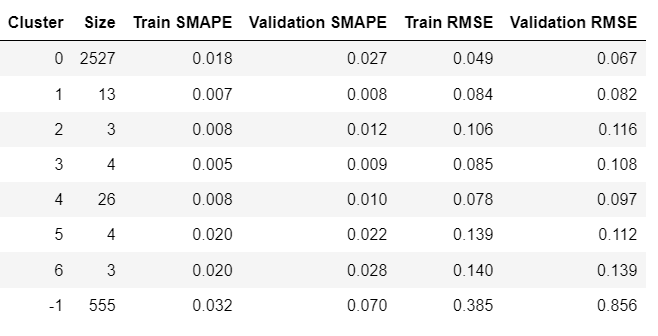
\includegraphics{images/lr_results2}
	\caption{LR model performance on each cluster ( after \textit{clipping} )}
\end{figure}

\subsection{Some Examples}

\begin{figure}[h]
	\centering
	\vspace{1em}
	\begin{subfigure}{0.45\textwidth}
		\animategraphics[autoplay,loop,width=\textwidth]{2}{images/lr_results/good_fit/fig_}{0}{10}
		\caption{Good Fit}
		\label{fig:lr_good}
	\end{subfigure}
	\begin{subfigure}{0.45\textwidth}
		\animategraphics[autoplay,loop,width=\textwidth]{2}{images/lr_results/poor_fit/fig_}{0}{10}
		\caption{Poor Fit}
		\label{fig:lr_poor}
	\end{subfigure}
	\caption{LR model performance visualization}
	\label{fig:lr_both}
\end{figure}

\subsection{Limitation(s) of model}
\vspace{1em}
\paragraph{Problem/Limitation} Linear regression didn't work effectively in some counties because there could have been some important predictor variables not included in the analysis, which could influence the microbusiness density. Additionally, the temporal dependency of time series is not considered, which could also affect the accuracy of the results. 
\paragraph{Solution} To address the issue of temporal dependencies in linear regression, we can use machine learning models that are specifically designed for time-series data, such as autoregressive integrated moving average (ARIMA) models, recurrent neural networks (RNNs), or long short-term memory (LSTM) models. These models can capture complex temporal dependencies and patterns in the data and can be used to forecast future microbusiness density values based on historical data.

\vspace{2em}
\section{\centering ARIMA Model}

\vspace{1em}
ARIMA models are frequently used to analyze time series data that demonstrate evidence of non-stationarity in their mean function (i.e., trend). This non-stationarity is characterized by a changing mean of the time series over time, which can make modeling and forecasting the series a challenging task.

\vspace{1em}
To mitigate this issue, ARIMA models include an ``Integrated" component. This component encompasses the differencing of the time series data one or more times to eliminate the trend and render the data stationary. Stationary data obtained after differencing has a constant mean and variance over time simplifies the modeling process because \textit{Wold's theorem} ensures that we can fit an ARMA model to that data. 

\textbf{Note}: Too much differencing can also introduce non-stationarity in data. Usually upto second order differencing is sufficient for most time series data. 

\vspace{1em}
\textbf{Wold's theorem} \cite{wold}, also known as the Wold decomposition theorem, is a fundamental result in time series analysis that states that any stationary time series can be represented as the sum of two components: a deterministic component and a stochastic component. The deterministic component can be represented by a linear function of past observations (AR part), while the stochastic component is a stationary process with uncorrelated errors (MA part). Overall, Wold's theorem provides a theoretical foundation for ARIMA model and helps to explain why they are effective for modeling stationary time series.


\vspace{1em}
The order of the ARIMA model is denoted by (p, d, q), where p represents the number
of past values used in the AR model, d represents the degree of differencing used, and q represents the number of past error terms used in the MA model



\vspace{1em}
\begin{center}
	\begin{tcolorbox}[colframe=orange,boxsep=5pt,boxrule=1pt,colback=white, width=0.8\linewidth]
		$
	(1 - \phi_1 L - \phi_2 L^2 - ... - \phi_p L^p)(1 - L)^d y_t = c + (1 + \theta_1 L + \theta_2 L^2 + ... + \theta_q L^q)\varepsilon_t		$
	\end{tcolorbox}
\end{center}

\vspace{1em}

\begin{itemize}
	\item $y_t$ is microbusiness density at time t 
	\item L is the lag operator, such that $L^i y_t = y_{t-i}$
	\item d is the order of differencing, such that $(1-L)^d y_t$ is the differenced time series of order d
	\item $\phi_1, ..., \phi_p$ are the autoregressive coefficients representing the dependence of $y_t$ on its p past values
	\item c is a constant term
	\item $\theta_1, ..., \theta_q$ are the moving average coefficients representing the dependence of $y_t$ on the q past error terms $\varepsilon_{t-1}, ..., \varepsilon_{t-q}$
	\item $\varepsilon_t$ is the current error term \textbf{assumed} to be independently and identically distributed with zero mean and constant variance
\end{itemize}

\subsection{Estimation of parameters and coefficients}

To find best parameters (p,d,q) of model we used brute force approach as we had both time and computation facility of HPC provided by IIT Goa.  To find best hyperparamters, we checked all possible 0 $\le$ p $\le$ 6 , 0 $\le$ d $\le$ 2 and 0 $\le$ q $\le$ 3 and picked the values which has minimum \textit{smape} error on both train data and validation data.  

\vspace{1em}
Once the values of p, d, and q have been determined, the coefficients ($\phi_1 \ldots \phi_p , \theta_1 \ldots \theta_q$ and c ) of the ARIMA model can be estimated using a technique called\textbf{ maximum likelihood estimation} (MLE) \cite{mle}. MLE involves finding the parameter values that maximize the likelihood of the observed data, given the model. The estimated coefficients can then be used to make forecasts for future values of the time series. To estimate the parameter values that maximize the likelihood function, numerical optimization algorithms such as gradient descent, Newton-Raphson method, or expected maximization(EM) algorithm can be used. The optimization algorithm iteratively adjusts the parameter values until the likelihood function is maximized. 

\vspace{1em}
\subsection{Results and Observations}

We have fitted the ARIMA model only on those counties which didn't perform well using linear regression and present results clusters-wise (after excluding already good-performing counties). To justify improvement, we presented the performance of linear regression on these counties. 

\vspace{1em}
In below table, we can see performance of the ARIMA model is better than Linear regression. It is because the linear regression algorithm does not consider the interdependence of micro-business density values from one month to the next, which the ARIMA model successfully captures.  

\vspace{1em}

\begin{figure}[h]
	\centering
	\vspace{1em}
	\begin{subfigure}{0.6\textwidth}
	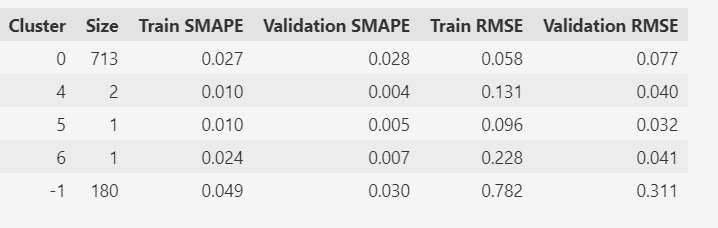
\includegraphics[width=\linewidth]{images/arima_results}
	\caption{ARIMA model}
	\label{fig:arima}
	\end{subfigure}

	\begin{subfigure}{0.6\textwidth}
	\centering
	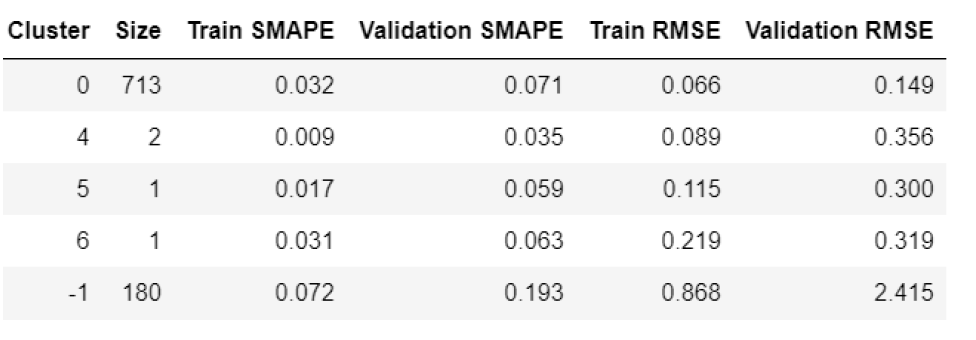
\includegraphics[width=\linewidth]{images/benchmark_arima_with_lr}
	\caption{LR model}
	\label{fig:lr_vs_arima}
	\end{subfigure}
	\caption{Comparing performance of ARIMA with LR}
	\label{fig:lr_arima_both}
\end{figure}

On closer look at predictions we find that out of 897 counties in updated clusters, 551 counties have smape error on training data less than 5\% and validation smape less than 2\%. so we will not consider those counties in next model.

\subsection{Some Examples}

\begin{figure}[h]
	\centering
	\vspace{1em}
	\begin{subfigure}{0.45\textwidth}
		\animategraphics[autoplay,loop,width=\textwidth]{2}{images/arima_results/good_fit/fig_}{0}{10}
		\caption{Good Fit}
		\label{fig:arima_good}
	\end{subfigure}
	\begin{subfigure}{0.45\textwidth}
		\animategraphics[autoplay,loop,width=\textwidth]{2}{images/arima_results/poor_fit/fig_}{0}{10}
		\caption{Poor Fit}
		\label{fig:arima_poor}
	\end{subfigure}
	\caption{ARIMA model performance visualization}
	\label{fig:arima_both}
\end{figure}

\subsection{Limitations(s) of model}

\paragraph{Limitations} The ARIMA model has several limitations that should be taken into account when considering its use for a particular application. One such limitation is the model's inability to handle long-term forecasting. While ARIMA is effective for short-term forecasting, its forecast accuracy decreases as the forecasting horizon increases, making it less suitable for longer-term predictions.

Additionally, the model struggles with seasonal data. Though it can be extended to include seasonality, this can be complex and requires additional parameters. Furthermore, ARIMA assumes a linear relationship between the dependent and independent variables, which means it cannot capture complex relationships and nonlinear patterns in the data. This can limit its forecasting accuracy, particularly when the relationship between variables is non-linear. 

\paragraph{Solution} To include seasonality, arima can be extended to sarima model explained in next section. Also to handle non-linear relationships we can use rnn or lstm based deep learning models.


\section{\centering SARIMA model}

SARIMA is extension of ARIMA model in sense that it also captures seasonal/periodic fluctuations in the data. SARIMA models can also handle time series data with inconsistent seasonal patterns by including additional parameters to capture the variability in the seasonality. The seasonal component of a SARIMA model includes a seasonal autoregressive (SAR) term, a seasonal difference (D) term, and a seasonal moving average (SMA) term.

\vspace{1em}
The SAR term captures the influence of the seasonal pattern in the previous season on the current season. The D term represents the number of seasonal differences needed to make the data stationary, and the SMA term captures the influence of the seasonal pattern in the previous season's forecast error on the current season's forecast.By including these additional seasonal parameters in the SARIMA model, it can capture more complex seasonal patterns, including cases where the seasonality is not consistent across different time periods.

\vspace{1em}
The SARIMA model is usually represented as SARIMA(p,d,q)(P,D,Q)s, where p, d,
and q are the order for the AR, I, and MA components, while P, D, and Q are the order for the seasonal AR, I, and MA components, and s is the seasonality period.


\vspace{1em}
\begin{center}
	\begin{tcolorbox}[colframe=orange,boxsep=5pt,boxrule=1pt,colback=white, width=1.1\linewidth]
		$
		(1 - \phi_1 L  - ... - \phi_p L^p)(1 - \Phi_1 L^s - ... - \Phi_P L^{Ps})(1 - L)^d (1 - L^s)^Dy_t = c + (1 + \theta_1 L + ... + \theta_q L^q)(1 + \Theta_1 L^s +  ... + \Theta_Q L^{Qs})\varepsilon_t		$
	\end{tcolorbox}
\end{center}

\vspace{1em}
\begin{itemize}
	\item $y_t$ is the observed value of the microbusiness-density at \textit{time\_step} $t$
	\item c is constant term
	\item $L$: the backshift operator, which shifts the time series by one period. In other words, $L*y_t = y_{t-1}$.
	\item $\phi_1, \phi_2, ..., \phi_p$: the non-seasonal autoregressive coefficients. 
	\item $\Phi_1, \Phi_2, ..., \Phi_P$: the seasonal autoregressive coefficients. 
	\item $(1-B)$: the non-seasonal difference operator. This operator is applied d times to the time series to remove the trend component.
	\item $(1-B^s)$: the seasonal difference operator. This operator is applied D times to the time series to remove the trend component.
	\item $\theta_1, \theta_2, ..., \theta_q$: the non-seasonal moving average coefficients. 
	\item $\Theta_1, \Theta_2, ..., \Theta_Q$: the seasonal moving average coefficients.
	\item $\varepsilon_t$ is the error term at \textit{time\_step} $t$,  which is assumed to be normally distributed with mean zero and constant variance.
\end{itemize}

\subsection{Estimation of parameters and coefficients}


Again, To find best parameters (p,d,q) of model we used brute force approach. To find best hyperparamters, we checked all possible 0 $\le$ p $\le$ 6 , 0 $\le$ d $\le$ 2 , 0 $\le$ q $\le$ 2, 0 $\le$ P $\le$ 2 , 0 $\le$ D $\le$ 2 and 0 $\le$ Q $\le$ 2 and s $\in$ \{6,12\} and picked the values which has minimum \textit{smape} error on both train data and validation data.  

\vspace{1em}
Once the values of p, d, q, P, D, Q and s have been determined, the coefficients ($\phi_1 \ldots \phi_p$ , $\theta_1 \ldots \theta_q$, $\Phi_1 \ldots \Phi_P$ , $\Theta_1 \ldots \Theta_Q$ and c ) of the SARIMA model are also estimated using method of \textbf{maximum likelihood estimation} (MLE).

\vspace{1em}
\subsection{Results and Observations}

On comparing results of SARIMA and ARIMA we see that SARIMA model is not performing
good on train data but it looks like it is performing better on validation data.


\vspace{1em}

\begin{figure}[h]
	\centering
	\vspace{1em}
	\begin{subfigure}{0.6\textwidth}
		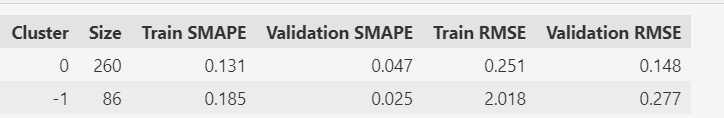
\includegraphics[width=\linewidth]{images/sarima_results}
		\caption{SARIMA model}
		\label{fig:arima}
	\end{subfigure}
	
	\begin{subfigure}{0.6\textwidth}
		\centering
		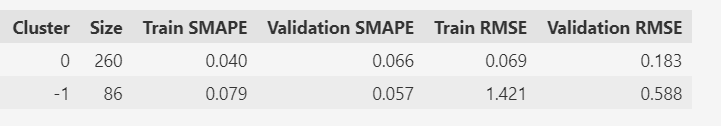
\includegraphics[width=\linewidth]{images/benchmark_sarima_with_arima}
		\caption{ARIMA model}
		\label{fig:sarima_vs_arima}
	\end{subfigure}
	\caption{Comparing performance of SARIMA with ARIMA}
	\label{fig:sarima_arima_both}
\end{figure}

On closer look at predictions we find that out of 346 counties in updated clusters 187 counties have validation smape less than 2\%. One thing that we observe is that about 41 counties ( approx. 25\% ) counties among worst performing counties have sudden spikes in micro-business at the end, This may be due to people trying to interfere with leaderboard of kaggle competition. Later, I will perform more extensive analysis on counties on which all models fail.

\vspace{1em}

\subsection{Some Examples}

\begin{figure}[h]
	\centering
	\vspace{1em}
	\begin{subfigure}{0.45\textwidth}
		\animategraphics[autoplay,loop,width=\textwidth]{2}{images/sarima_results/good_fit/fig_}{0}{1}
		\caption{Good Fit}
		\label{fig:sarima_good}
	\end{subfigure}
	\begin{subfigure}{0.45\textwidth}
		\animategraphics[autoplay,loop,width=\textwidth]{2}{images/sarima_results/poor_fit/fig_}{0}{1}
		\caption{Poor Fit}
		\label{fig:sarima_poor}
	\end{subfigure}
	\caption{SARIMA model performance visualization}
	\label{fig:sarima_both}
\end{figure}


\subsection{Limitation(s)  of model}

\paragraph{Limitation} SARIMA assumes a linear relationship between past and future values. However, many time series have nonlinear patterns that are difficult to capture using linear models like SARIMA. 

\paragraph{Solution} To capture non-linearity in model we tried out two models : XGBoost and RNN explained in next sections. 

\newpage
\section{\centering XGBoost Model}
\vspace{1em}

\textbf{\textit{Pre-requisites:}}
\begin{itemize}
	\item Ensemble learning
	\item Decision Trees
\end{itemize}

\subsection{Ensemble Learning}
\vspace{1em}

\paragraph{Ensemble learning}is a machine learning technique that combines multiple models to produce a more accurate and robust prediction. The basic idea behind ensemble learning is that by combining the predictions of multiple models, we can reduce the impact of errors or biases in any single model and produce a more accurate prediction overall. The most common types of ensemble learning are \textbf{bagging}, \textbf{boosting}, and \textbf{stacking}. 


\paragraph{Bagging}( Bootstrapped aggregating ) is a technique that involves training multiple models on randomly selected subsets of training data. The final prediction is the average of the predictions of all the models. 

\paragraph{Boosting} involves training multiple models sequentially, with each model correcting the errors of the previous model. In boosting, each model is trained on residuals of the previous model, and the final prediction is the weighted sum of individual model predictions. 

\paragraph{Stacking} involves combining predictions of multiple base models using a \textit{meta-model}. In stacking, each base model is trained on the same training data, and the final prediction is made by \textit{meta-model} that takes the predictions of base models as input. The meta-model learns to combine the predictions of base models in a way that maximizes their strengths and minimizes their weaknesses. 

\vspace{1em}
In this competition, since the dataset is relatively small ( 41 observations for each county ), we will use the \textit{boosting} technique, more specifically \textbf{extreme gradient boosting} (xgboost) technique which is explained later.

\subsection{Decision Trees}
\vspace{1em}



\paragraph{Decision Tree} is a tree-like model for making decisions based on certain conditions. It consists of nodes that represent conditions and branches that represent the possible outcomes. At each node, a decision is made based on a set of conditions until a leaf node is reached, which represents the final decision.In this competition, since time series in a continuous data, we will be building so called \textit{regression trees} which is just fancy name for decision tree using continuous variable at each node. 

\newpage
\begin{figure}[h]
	\centering
	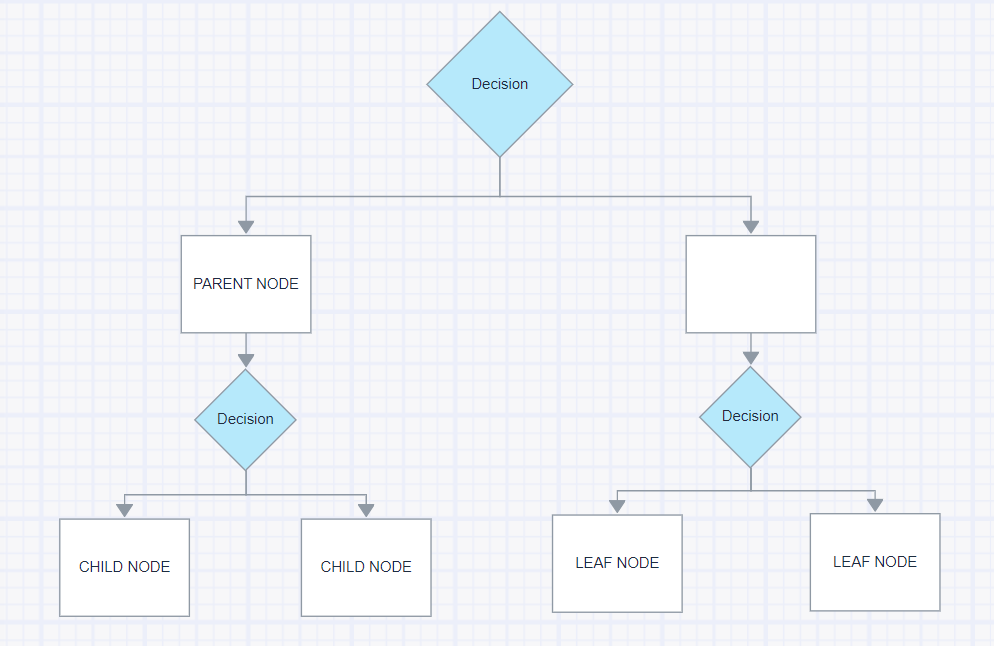
\includegraphics[scale=0.6]{images/decision_tree}
	\caption{Decision Tree}
\end{figure}

\vspace{1em}
\paragraph{Construction of decision Tree } 

\vspace{1em}
A regression tree is constructed by recursively partitioning the data into subsets based on a similarity score and a gain criterion. Here's how it works:

\begin{itemize}
	\item \textbf{\textit{Similarity Score}}: The first step is to select a similarity score that measures the similarity between the input variables and the target variable. A common similarity score used for regression tasks is the sum of squared errors, which measures the difference between the predicted and actual values.
	
	The similarity score, $S$, is calculated as the sum of squared errors between the predicted value $\hat{y}$ and the actual value $y$:
	
	$$ S = \sum_{i=1}^{n} ( y_i - \hat{y_i})^2 $$
	
	\item \textit{\textbf{Gain Criterion}}: The next step is to select a gain criterion that measures the improvement in the similarity score after splitting the data into subsets. A common gain criterion used for regression trees is the mean squared error reduction, which measures the reduction in the sum of squared errors after splitting the data.
	
	The gain criterion, $G$, is calculated as the difference between the similarity score before and after splitting the data:
	
	$$ G = S - \frac{S_1 + S_2}{2} $$
	
	\item \textit{\textbf{Splitting the Data}}: The regression tree algorithm then selects the input variable and the threshold value that maximize the gain criterion by checking all possible threshold values which could split the data into two subsets. The data is split into two subsets based on whether the input variable is above or below the threshold value.
	
	\item \textit{\textbf{Output Value}}: Once the data is split, the algorithm calculates the output value for each subset. The output value is typically the mean of the target variable within the leaf node.
	
	The output value, $\hat{y}$, is typically the mean of the target variable within leaf node:
	
	$$ \hat{y} = \frac{1}{r} \sum_{i=1}^{r} y_i $$
	
	\item\textit{\textbf{ Recursion}}: The algorithm then recursively applies the same procedure to each subset until a stopping criterion is met, such as reaching a maximum depth or a minimum number of samples in each leaf node. 
\end{itemize}

\vspace{1em}
\subsection{XGBoost}

\paragraph{Gradient boosting} is a machine learning technique that combines multiple weak predictive models like decision trees into a single strong predictive model. It works by iteratively adding weak models to the ensemble, each one trained to correct the errors of the previous models. At each iteration, the algorithm calculates the residuals and trains a new model to fit these residuals. Specifically, In gradient boosting residuals are defined as negative gradient of loss function with respect to predictions which is nothing but first order approximation of taylor series expansion of loss function. 

\paragraph{XGBoost} is an optimized implementation of gradient boosting that uses a number of
advanced techniques to improve its performance and scalability. These include:

\begin{itemize}
	\item \textbf{\textit{Tree pruning}}: removing branches that do not contribute to the overall accuracy of the	model, to reduce over-fitting.
	\item \textbf{\textit{Hardware optimization}}: using parallel processing and cache-aware algorithms to speed up training.
	\item \textbf{\textit{Regularization}}: adding penalties to the loss function to prevent overfitting and improve generalization	etc.
\end{itemize}

\subsection{Results and Observations}


\vspace{1em}

\begin{figure}[h]
	\centering
	\vspace{1em}
	\begin{subfigure}{0.6\textwidth}
		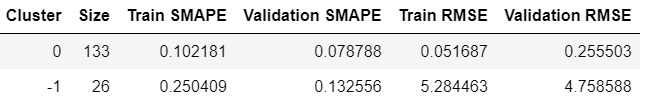
\includegraphics[width=\linewidth]{images/xgboost_results}
		\caption{XGBoost model}
		\label{fig:arima}
	\end{subfigure}
	
	\begin{subfigure}{0.6\textwidth}
		\centering
		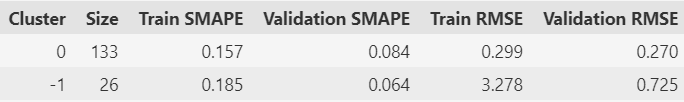
\includegraphics[width=\linewidth]{images/benchmark_xgboost_with_sarima}
		\caption{SARIMA model}
		\label{fig:sarima_vs_arima}
	\end{subfigure}
	\caption{Comparing performance of XGBoost with SARIMA}
	\label{fig:sarima_arima_both}
\end{figure}

XGBoost model is performing better on Cluster 0 but its performance on Cluster -1 is
worse than SARIMA model. On closer look at predictions, we noticed 82 counties have validation smape less than 5\% ( which is reasonable threshold in this case because after visually inspecting we found model is generalizing well on these counties).


\newpage
\subsection{Some Examples}


\begin{figure}[h]
	\centering
	\vspace{1em}
	\begin{subfigure}{0.45\textwidth}
		\animategraphics[autoplay,loop,width=\textwidth]{2}{images/xgboost_results/good_fit/fig_}{0}{1}
		\caption{Good Fit}
		\label{fig:xgboost_good}
	\end{subfigure}
	\begin{subfigure}{0.45\textwidth}
		\animategraphics[autoplay,loop,width=\textwidth]{2}{images/xgboost_results/poor_fit/fig_}{0}{1}
		\caption{Poor Fit}
		\label{fig:xgboost_poor}
	\end{subfigure}
	\caption{XGBoost model performance visualization}
	\label{fig:xgboost_both}
\end{figure}


\subsection{Limitation(s) of model}

Even though model is able to capture some non-linear relationship but it can only predict in range, it has already seen. also model is not able to learn sudden jumps in microbusiness density. we will solve that problem using rnn based models as explained in next section. 

\vspace{2em}
\section{\centering Recurrent Neural Networks}
\vspace{1em}

A \textbf{Recurrent Neural Network} (RNN) is a type of neural network that is designed to process sequential data. Unlike traditional neural networks that only process input data in a single forward pass, RNNs can also process data with a temporal dimension, such as time-series data or text.

\begin{figure}[h]
	\centering
	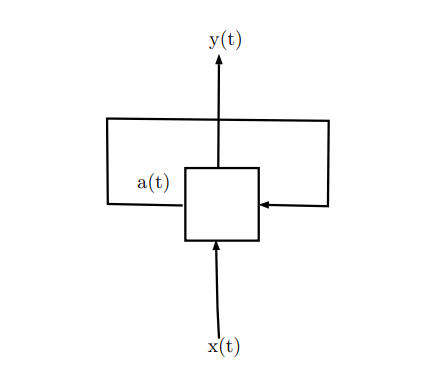
\includegraphics[scale=0.8]{images/rnn_unit}
	\caption{RNN unit}
\end{figure}

\paragraph{Intuition} The key intuition behind an RNN is that it maintains an internal state or memory that allows it to process inputs in a sequential order. At each time step, the RNN takes in an input and uses its current internal state to produce an output. The output is then fed back into the RNN as the input for the next time step, along with a new input. This feedback loop allows the RNN to build up a representation of the entire sequence of inputs it has seen so far.


\paragraph{Applications} RNNs are useful in a wide range of applications, such as speech recognition, language modeling, and sentiment analysis. They are particularly useful when the input data has a temporal dimension or exhibits temporal dependencies, since they can capture and use information from previous inputs to inform the processing of current inputs.

\vspace{1em}
\begin{figure}[h]
	\centering
	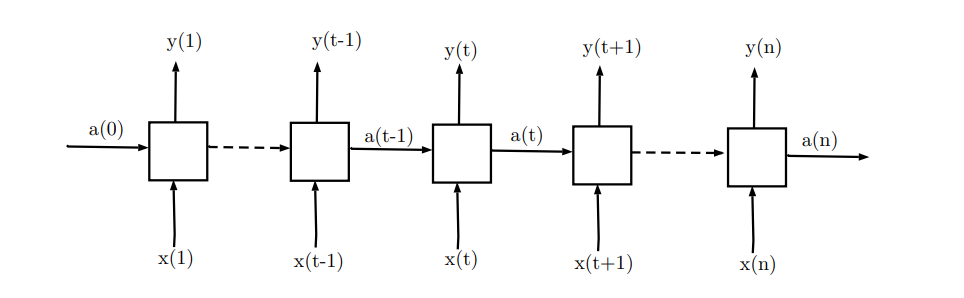
\includegraphics[scale=0.8]{images/rnn_unfolded}
	\caption{Unfolded RNN unit}
\end{figure}

\paragraph{Mathematically } A RNN can be represented by following set of equations 
\begin{center}
\begin{tcolorbox}[colframe=orange,boxsep=5pt,boxrule=1pt,colback=white, width=0.6\linewidth]
\begin{equation*}
	\begin{aligned}
		\centering
		&a(t) = g_1 ( W_{aa} * a(t-1) + W_{ax} * x(t) + b_a)\\
		&y(t) = g_2 ( W_{ya} * a(t) + b_y )
	\end{aligned}
\end{equation*}
\end{tcolorbox}
\end{center}

\hspace{1em} here $g_1$ and $g_2$ are activation functions and * denotes element-wise multiplication and $W_{aa}$, $W_{ax}$, $W_{ya}$, $b_a$, $b_y$ are coefficients that are shared temporally. since same weights are used across all time stamps, it can be treated as single neuron with a feedback mechanism which takes different inputs ( x(t), a(t-1)) at each time step , hence the word ”recurrent” in the name of RNNs.


\subparagraph{Limitation} One main challenge with training RNN is vanishing gradient problem. It occurs when during back-propagation step for updating network parameters , gradient of loss function become too small due to repeated multiplication of activation function (e.g. sigmoid function ) . 


\paragraph{Variations of RNN} To overcome above limitation, several variations of RNNs have been developed. In particular, for time series data where we want to predict future values based on past data which have temporal dependencies , two most commonly used RNN architectures are Long Short Term Memory (\textbf{LSTM}) and Gated Recurrent Unit (\textbf{GRU}) which are explained in next section. 

\paragraph{Gates in RNNs} RNN variations like LSTM and GRU uses gating mechanism to avoid vanishing gradient problem . These so called \textbf{Gates} introduce additive property in calculation of gradient of loss function which in turn ensure gradients in back-propagation step are significant. Gates are usually denoted by T and are equal to 


\begin{center}
\begin{tcolorbox}[colframe=orange,boxsep=5pt,boxrule=1pt,colback=white, width=0.6\linewidth]
\begin{equation*}
	\centering 
	T = \sigma ( W * x (t)  + U * a(t-1) + b )
\end{equation*}
\end{tcolorbox}
\end{center}


where W, U, b are constants specific to gate and $\sigma$ is sigmoid function. 


\vspace{2em}
\begin{table}[h]
	\centering
	\caption{\textbf{Types of Gates}}
	\begin{tabular}{|c| c | c|}
		\hline
		\textbf{Gate Name} & \textbf{Symbol} & \textbf{Role} \\
		\hline
		Update gate & $T_u$ & Decides how much past should matter now \\
		\hline 
		Reset gate & $T_r$ & Decides how much to drop the previous information \\
		\hline 
		Forget gate & $T_f$ & Decides how much to erase a cell state \\
		\hline 
		Output gate &  $T_o$ & Decides how much to reveal of a cell state to next layer \\
		\hline
	\end{tabular}
\end{table}

\subsection{Long Short Term Memory}

\textbf{Long Short-Term Memory} (LSTM) is a type of recurrent neural network  architecture that was designed to overcome the limitations of traditional RNNs in capturing long-term dependencies in sequential data. The architecture of LSTM includes three types of gates: the input gate, forget gate, and output gate, each of which controls the flow of information through the network


\subsubsection{Architecture}
\vspace{1em}
\begin{figure}[h]
	\centering
	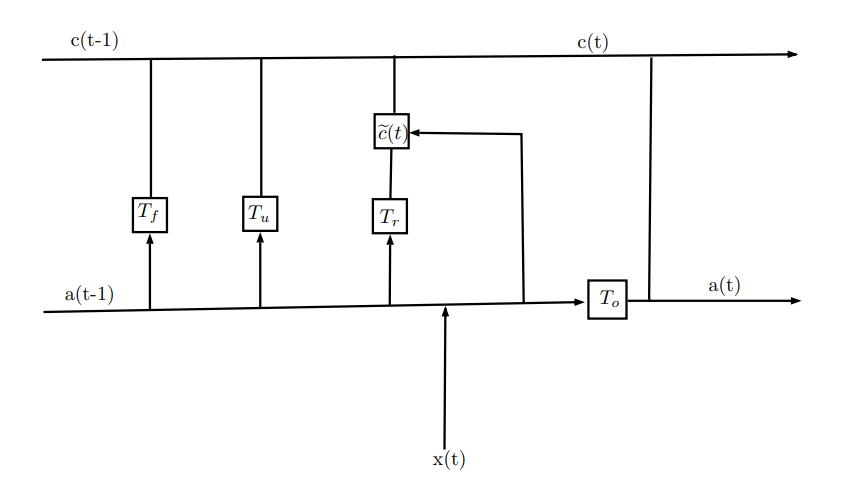
\includegraphics[scale=0.75]{images/lstm}
	\caption{Architecture of LSTM}
\end{figure}


\subsubsection{Mathematical Formulation}

\vspace{1em}

\begin{center}
\begin{tcolorbox}[colframe=orange,boxsep=5pt,boxrule=1pt,colback=white, width=0.6\linewidth]
\begin{equation*}
	\begin{aligned}
		\centering
		& \tilde{c}(t) = tanh( W_c [T_r * a(t-1), x(t)] + b_c)	\\
		& c(t) =  T_u * \tilde{c}(t) + T_f * c(t-1) \\
		& a(t) =  T_o * c(t) \\
	\end{aligned}
\end{equation*}
\end{tcolorbox}
\end{center}

\hspace{1em} In summary these equation demonstrate following : 

\begin{itemize}
	\item $\tilde{c}(t)$ is the \textbf{new candidate cell state}, which depends on the current input and previous hidden state 
	
	\item $c(t)$ is the \textbf{updated cell state}, which depends on candidate cell state and  previous cell state 
	
	\item $a(t)$ is the \textbf{output hidden stat}e, which depends on current cell state. 
	
	\item At each step different gates are applied as required. 
\end{itemize}


\hspace{1em} The LSTM architecture uses these equations to selectively store, forget, and update information in the cell state over time, allowing the model to handle long-term dependencies in sequential data.


\subsubsection{Results and Observations}

\begin{figure}[h]
	\centering
	\vspace{1em}
	\begin{subfigure}{0.6\textwidth}
		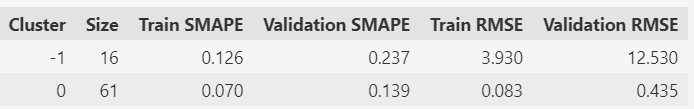
\includegraphics[width=\linewidth]{images/lstm_results}
		\caption{LSTM model}
		\label{fig:lstm}
	\end{subfigure}
	
	\begin{subfigure}{0.6\textwidth}
		\centering
		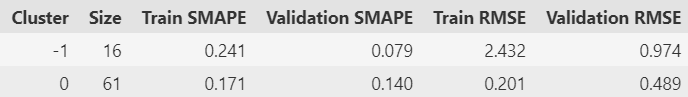
\includegraphics[width=\linewidth]{images/benchmark_lstm_with_sarima}
		\caption{SARIMA model}
		\label{fig:lstm_vs_sarima}
	\end{subfigure}
	\caption{Comparing performance of LSTM with SARIMA}
	\label{fig:lstm_sarima_both}
\end{figure}

Clearly, Overall LSTM model is not performing well on validation data but is fitting quite good on training data. Infact on closer look we did found some counties where LSTM outperforms SARIMA. 

On close inspection we observed that around \textbf{35} performance have improved when compared with SARIMA model results. It is happening because LSTM model is able to capture sudden jumps as can be seen in Figure ~\ref{fig:lstm_good}. 

\newpage
\subsubsection{Some Examples}

\begin{figure}[h]
	\centering
	\vspace{1em}
	\begin{subfigure}{0.45\textwidth}
		\animategraphics[autoplay,loop,width=\textwidth]{2}{images/lstm_results/good_fit/fig_}{0}{1}
		\caption{Good Fit}
		\label{fig:lstm_good}
	\end{subfigure}
	\begin{subfigure}{0.45\textwidth}
		\animategraphics[autoplay,loop,width=\textwidth]{2}{images/lstm_results/poor_fit/fig_}{0}{1}
		\caption{Poor Fit}
		\label{fig:lstm_poor}
	\end{subfigure}
	\caption{LSTM model performance visualization}
	\label{fig:lstm_both}
\end{figure}



\subsection{Gated Recurrent Unit}

\vspace{1em}

\textbf{Gated Recurrent Unit}(GRU) is similar to the more well-known LSTM network however the GRU is simpler than LSTM and has fewer parameters, making it easier to train and faster to run. The GRU also has a smaller memory footprint, which can be an advantage in applications with limited computational resources.

\vspace{1em}
\subsubsection{Architecture}
\vspace{1em}
\begin{figure}[h]
	\centering
	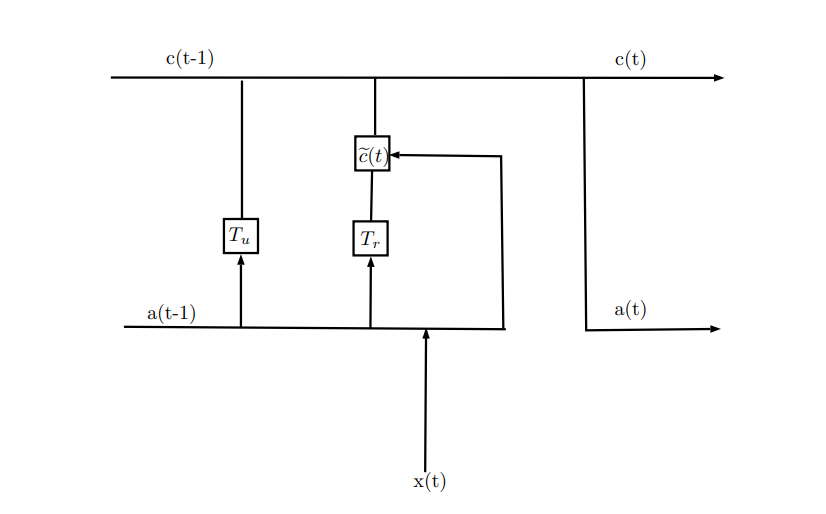
\includegraphics[scale=0.7]{images/gru}
	\caption{Architecture of GRU}
\end{figure}

\newpage
The key innovation of the GRU is the use of two gates: an update gate and a reset gate. The update gate controls how much of the previous hidden state should be retained and how much of the new input should be added to the hidden state. The reset gate controls how much of the previous hidden state should be ignored when computing the new hidden state.

\vspace{1em}
\subsubsection{Mathematical Formulation}
\vspace{1em}

\begin{center}
\begin{tcolorbox}[colframe=orange,boxsep=5pt,boxrule=1pt,colback=white, width=0.6\linewidth]
\begin{equation*}
	\begin{aligned}
		\centering
		& \tilde{c}(t) = tanh( W_c [T_r * a(t-1), x(t)] + b_c)	\\
		& c(t) =  T_u * \tilde{c}(t) + (1 - T_u) * c(t-1) \\
		& a(t) =  c(t) \\
	\end{aligned}
\end{equation*}
\end{tcolorbox}
\end{center}

Symbols meaning is same as explained in LSTM section. 

\vspace{1em}
\subsubsection{Results and Observations}


\begin{figure}[h]
	\centering
	\vspace{1em}
	\begin{subfigure}{0.6\textwidth}
		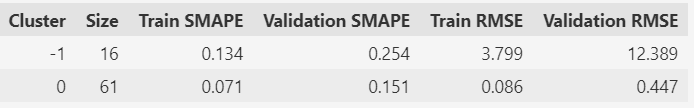
\includegraphics[width=\linewidth]{images/gru_results}
		\caption{GRU model}
		\label{fig:gru}
	\end{subfigure}
	
	\begin{subfigure}{0.6\textwidth}
		\centering
		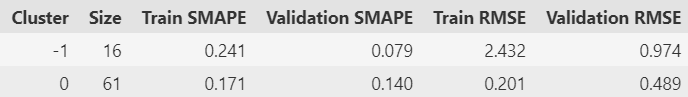
\includegraphics[width=\linewidth]{images/benchmark_lstm_with_sarima}
		\caption{SARIMA model}
		\label{fig:gru_vs_sarima}
	\end{subfigure}
	\caption{Comparing performance of GRU with SARIMA}
	\label{fig:gru_sarima_both}
\end{figure}

Similar to LSTM, GRU model also outperform SARIMA in around 31 counties. On close inspection we saw these counties infact same counties we found while analyzing LSTM  results. 

\newpage
\subsubsection{Some Examples}

\begin{figure}[h]
	\centering
	\vspace{1em}
	\begin{subfigure}{0.45\textwidth}
		\animategraphics[autoplay,loop,width=\textwidth]{2}{images/gru_results/good_fit/fig_}{0}{1}
		\caption{Good Fit}
		\label{fig:lstm_good}
	\end{subfigure}
	\begin{subfigure}{0.45\textwidth}
		\animategraphics[autoplay,loop,width=\textwidth]{2}{images/gru_results/poor_fit/fig_}{0}{1}
		\caption{Poor Fit}
		\label{fig:lstm_poor}
	\end{subfigure}
	\caption{GRU model performance visualization}
	\label{fig:lstm_both}
\end{figure}


\section{Summary}

\vspace{2em}
\begin{table}[h]
	\centering
	\caption*{\textbf{Overall Models Performance}}
	\begin{tabular}{|c| c | c| c | c |}
		\hline
		\textbf{Model} & \textbf{Benchmark Model} & \textbf{Counties} & \textbf{SMAPE} & \textbf{Benchmark SMAPE}  \\
		\hline
		Linear Regression & NA & 3135 & 0.034 & NA \\
		\hline
		ARIMA & Linear Regression & 897 & 0.028 & 0.090 \\
		\hline
		SARIMA & ARIMA & 346 &  0.041 & 0.059 \\
		\hline
		SARIMAX & SARIMA & 159 & 0.113 &  0.080 \\
		\hline
		XGBoost & SARIMA &  159 & 0.087 & 0.080 \\
		\hline
		LSTM & SARIMA & 77 & 0.159 & 0.127 \\
		\hline
		GRU & SARIMA & 77 & 0.172 & 0.127 \\
		\hline
	\end{tabular}
\end{table}

\vspace{1em}
In this BTech project we used various time-series technique learned as part of our \textbf{Time Series Analysis} course like ARIMA, SARIMA etc. We applied these algorithms/technique on a real-world time series data. Apart from this we also saw limitations of these models and tried some standard machine learning methods like Linear regression, XGBoost and Neural network architecture like LSTM and GRU. 

\vspace{1em}
Through this project, We developed a strong understanding of time series forecasting techniques and was able to apply them to a real-world problem. Using multiple models allowed us to evaluate the strengths and weaknesses of each approach and identify which models were most effective for the given data set.

\vspace{1em}
Overall, this B.Tech project allowed me to demonstrate my technical skills and showcase my ability to apply time series forecasting techniques to real-world problems. It has equipped me with valuable skills that I can use in a wide range of industries and fields. 


\bibliographystyle{unsrt}
\nocite{rnn_article,stat_quest}
\bibliography{references}


\end{document}
